
\begin{center}
    \begin{figure}
    \makebox[\textwidth]{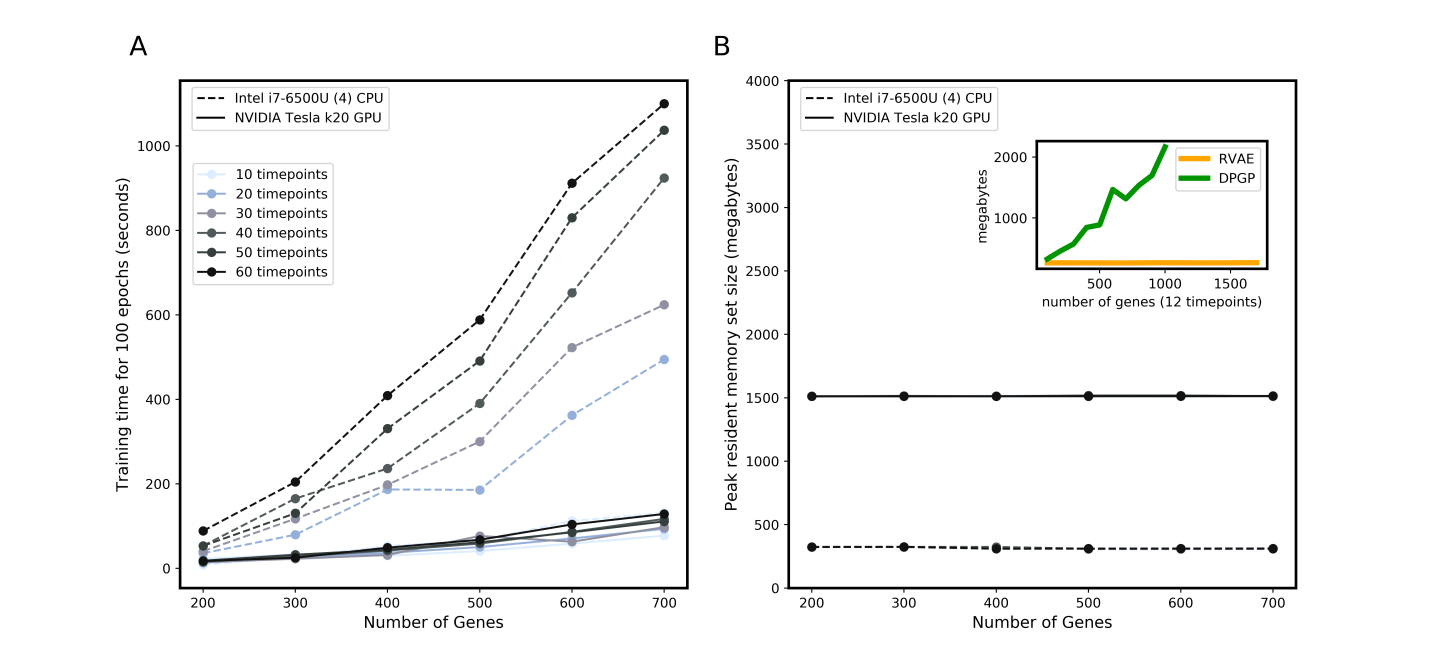
\includegraphics[width=0.8\paperwidth]{figures/fig7.png}}
 % archetecture.png: 1149x508 px, 72dpi, 40.53x17.92 cm, bb=0 0 1149 508
        \caption[Computational cost of training RVAgene]{\textbf{Training RVAgene is reasonably scalable on CPU and even more so using hardware acceleration through GPU.} ({\bf A}) Time cost of training RVAgene for 100 epochs for datasets with varying number of genes and time points on CPU and GPU. ({\bf B}) Maximum memory utilized during training of the model on CPU an GPU for the cases in (A), inset plot: comparison of max memory used compared to DPGP for varying number of genes.}
  \label{fig:fig7}
\end{figure}
\end{center}


\subsection{Assessment of the computational efficiency of RVAgene}

We assessed the computational efficiency of RVAgene for various settings and hardware. For the majority of the models trained, 100-200 epochs was sufficient for the loss function $\cL$ to converge. For tests performed here, we recorded the RVAgene runtime for 100 epochs of training using models that varied in their number of genes and time points. In each case we used a latent space of dimension two, a hidden size of 10, and a training batch size of 10. We ran the model on an intel i7 CPU with four cores and a Tesla K20 GPU. Runtimes were recorded on linux via the inbuilt time script (\texttt{/usr/bin/time --verbose}). As the number of time points and genes grew large (up to 60 time points and 700 genes), total runtimes on CPU were on the order of $10^3$ seconds ($<$ 20 minutes) (\hyperref[fig:fig7]{Fig. 6A}). On GPU, total runtimes were decreased to around $100$ seconds ($< 3$ minutes). Thus, RVAgene is readily scalable to tens of thousands of genes and hundreds of time points for training times of up to a few days on CPU or hours on GPU. For comparison, as described in \citet{McDowell2018}, the approximation-free time complexity of each iteration of learning for DPGP is $\cO(GT^3)$, due to the $G$ matrix inversions, each of size $T \times T$, for a dataset with $G$ genes and $T$ timepoints. The complexity for each epoch of training of RVAgene is $\cO(GT)$.
%The cubic complexity of the hierarchical Gaussian Process learning in DPGP quickly increases training time and does not allow scalability over timepoints without some form of approximation.
\par 
In terms of peak memory usage, since RVAgene is a neural network trained using backpropagation  \citep{rumelhart1986learning}, maximum memory used during training is of the same size as the network itself, which is constant given that the model parameters are fixed  (\hyperref[fig:fig7]{fig. 6B}). This is in contrast to Gaussian Processes (such as DPGP), which initially assign each gene to its own cluster, thus must store $G$ matrices of size $T\times T $, for $G$ genes and $T$ timepoints per gene. This leads to quickly increasing runtime peak resident set sizes for DPGP compared to RVAgene (\hyperref[fig:fig7]{fig. 6B} Inset). The memory used by DPGP grows with the number of time points as $\cO(GT^2)$). Thus, DPGP will not run with large numbers of genes and time points. %, and RVAgene has greater potential for the discovery of nuanced dynamical features in the data.
A note on this comparison: it is not direct, in the sense that DPGP performs clustering and RVAgene does not, in addition to other important differences between the goals of the methods. 
%However, we must add that direct comparisons must be made cautiously, given the differences between the two methods. 
%DPGP performs independent gene clustering; RVAgene does not (clustering can be performed downstream on the latent space).
Nonetheless, the size and scope of current biological datasets -- particularly at single-cell resolution -- in many cases preclude the use of DPGP without large reductions of the input data size. As we have shown, a feasible and efficient alternative in such cases is to run RVAgene, and then to perform clustering or other classification analyses post hoc on the latent space of the model. 

